\section{Methodology}
\subsection{Dataset}
The dataset used for this project is the Bonn University EEG dataset, which contains data from five healthy subjects as well as 5 subjects suffering from epilepsy \cite{bonnData}. The ten subjects have been measured using single-channel EEG measurements, which are then split in to five subsets, A through E. The healthy subjects had measurements taken with their eyes opened and closed, which are set A and B, respectively. Sets C and D were measured from the epilepsy patients, while they were not experiencing an active seizure, but with two different electrode placements. The final set, E, was recorded from the epilepsy patients while they were experiencing an active seizure. The data was recorded in segments of 23.6 seconds at a sampling frequency of 173.61 Hz, giving 4097 datapoints per measurement, and each subset contains 100 measurements. All measurements inside each subset have been randomized, such that they cannot be connected by their sequence in the dataset. 
For this project only classification of healthy vs active seizure subjects is considered, so only the subsets A, B and E are used. It should be noted that this gives an unbalanced dataset, as there are twice as many healthy measurements as active seizure ones. A plot of one measurement from each of these subsets can be seen in \cref{fig:EEG_data}. 

\begin{figure}
    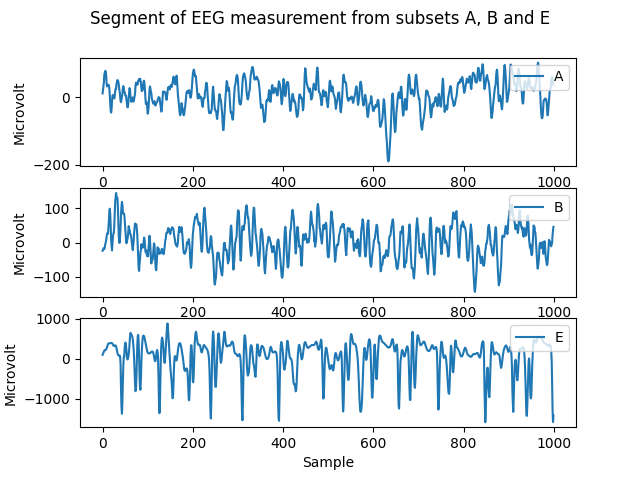
\includegraphics[width=\textwidth]{figures/EEG_data_vis.png}
    \caption{Plot of one measurement from each of the subsets A, B and E.}
    \label{fig:EEG_data}
\end{figure}
\subsection{Data preprocessing}
Minimal preprocessing is done on the data in this project, as the intention is for the model to be trained on the time-series data. A bandpass filter is applied to the data with a passband og $0.5$ Hz to $40$ Hz, this is to remove any artifacts created during data collection. Each data point is then normalized to its z-score, this is done because the model which is going to be used, a convolutional neural network, is very sensitive to large differences in magnitude, so if other patterns are to be found, those differences need to be removed. 

\subsection{Model architecture}
The chosen model architecture for this task is a combined convulational neural network and a long short-term memory (CNN-LSTM) model. 
The idea behind this is that the CNN model will be applied to the input data, where it will attempt to find spatial features in the input, as the convolutional filters are passed over it. 
The CNN in this paper is implemented with this structure:
\begin{minted}[breaklines]{python}
# CNN feature extractor
self.cnn = nn.Sequential(
    nn.Conv1d(1, cnn_internal, kernel_size=kernel_size1, stride=1, padding=kernel_size1//2),
    nn.ReLU(),
    nn.MaxPool1d(2),
    nn.Dropout(dropout),

    nn.Conv1d(cnn_internal, cnn_out, kernel_size=kernel_size2, padding=kernel_size2//2),
    nn.ReLU(),
    nn.MaxPool1d(2),
    nn.Dropout(dropout)
)
\end{minted}
The convolutional 1D layers detect spatial features, the ReLU activation layers introduce non-linearities and prevent vanishing gradient problems, the max pooling layers serve to only forward the most significant features while also halving the output size, such that the LSTM will be operating on an input one quarter the size of the input to the CNN. The dropout layers help in preventing overfitting to the training data. A grid search will later be performed to find the best kernel sizes and layer sizes etc. {\color{red} Skal der stå mere eller mindre her????}

The output values, i.e. what features were found and their spatial locations, are then passed in to the LSTM model, which attempts to learn what a sequence of features over time signifies. Each output feature of the CNN is passed in to the LSTM separately, so it learns on the features over time. A fully connected layer is then used to connect the output of the LSTM to the two output classes.

\subsection{Data segmentation}
To increase the amount of data available for training, and to decrease the size of the input to the model, all measurements are segmented in to segments of 1 second duration. This segmentation can be done without degrading the quality of the training data, as the classification is more about detecting a state, the state of having a seizure, and not so much about the long running structure of the data. 
To further increase the amount of training data, all training data segments also overlap, such that 2 seconds of measurement can become five 1 second segments, with an overlap of $75$\%. This overlap also should increase detection capability, as the model learns to recognize seizure markers not by their position in the input data, but only by the characteristica of the surrounding data.
Test and validation data also gets segmented, but without overlap, as there is no need to inflate the amount of data in these sets.

\subsection{Model training}
For training the model a cross entropy loss function is used as the criterion, where the initial weights of the criterion are loaded with double value for the active seizure class, which has half as many samples as the healthy class.
For optimization an adaptive moment (Adam) optimizer is used, which combines the adaptive learning rate of root mean square propagation with the convergence speed of momentum based optimization. The Adam optimizer will adjust learning rates for each individual weight that is being trained in the model, reducing the rate if the gradient starts oscillating.
To reduce oscillations in the overall model's validation loss, a learning rate scheduler is used, which will reduce the learning rate, if the validation loss hits a plateau, in the hopes that that will bring the model closer to the local minimum that it is oscillating around.

To prevent the model overfitting to the training data an early stopping class is also implemented, which looks at the validation loss after each epoch, and saves the model parameters each time it improves. If the validation loss does not improve for a number of epochs, model training is stopped, and the model weights with the best validation loss are loaded before evaluation.

To find the best model hyper-parameters, a grid search is executed, training a large number of models on many different combinations of parameters. Each model is evaluated with hold-out validation, and then all performance metrics and parameters are saved. The saved performance metrics are F1-score, accuracy, precision, recall and confusion matrix. The F1-score will be used to determine the best model, as that strikes a balance between penalizing both false positives and false negatives, as both are important when trying to detect seizures. 

{\color{red} skriv noget om data leakage måske?}


Describe the model architecture, dataset, pre-processing steps (if any), training strategy details (optimizer, loss, etc.), evaluation metrics, and implementation details. Please make sure that all the figures should be clear and must have a caption. Further, equations should be numbered correctly. Also, all the variables in the equations should be explained.

About 2 pages.